\section{Efficiency}
In general, the efficiency of a given detector system is estimated by using
information from other systems to select a set of ``clean'' events that can
reasonably be expected to produce a signal in that particular system.
Let $N^{should}$ be the number of events selected by a cut $C^{should}$ that
should show a signal in detector $D$, and $N^{did}$ be the subset of those
events that pass a cut $C^{did} = C^{should} \land C^{D}$,
where $C^{D}$ is an additional cut on information from the detector
$D$ under consideration and $\land$ represents the logical operation
\textit{and}.
Then the efficiency of $D$ is $\epsilon^D = N^{did}/N^{should}$.

\subsection{HMS Calorimeter} \label{sec:hcal_eff}
A set of electrons that should have normalized track energy deposition
approximately equal to one are selected using the cuts in
Table~\ref{tab:hcal_cuts}.

\begin{table}[h]
    \centering
    \caption{List of cuts used to estimate HMS Calorimeter efficiency.}
    \label{tab:hcal_cuts}
%      \begin{tabular}[t]{| c | l | l |}
    \begin{tabular}[t]{ c  l  l }
\specialrule{.1em}{.05em}{.05em} %\hline \hline
                   &  Variables              &  Cut \\
\specialrule{.1em}{.05em}{.05em}
        \multirow{4}{*}{\makecell[ml]{$C^{should}$}}
        &  HMS Cherenkov NPE      &  H.cer.npeSum>0                         \\ \cline{2-3}
        &  $\delta_{HMS}$         &  -10.0 < H.gtr.dp \&\& H.gtr.dp < 10.0  \\ \cline{2-3}
        &  $\beta_{HMS}$          &  0.8 < H.gtr.beta \&\& H.gtr.beta < 1.2 \\ \cline{2-3}
        &  Good hodoscope time    &  H.hod.goodstarttime==1                 \\
\specialrule{.1em}{.05em}{.05em}
        \multirow{2}{*}{\makecell[ml]{$C^{HCal}$}}
        &  HMS Calorimeter Energy &  \makecell{0.8 < H.cal.etottracknorm \&\&  \\
                                               H.cal.etottracknorm < 1.15} \\
\specialrule{.1em}{.05em}{.05em}
    \end{tabular}
\end{table}

Events are divided into $\delta$ bins of width 5 and efficiencies
$\epsilon_i=N_i^{did}/N_i^{should}$ are calculated for each bin.
A 95\% confidence interval for each bin's estimated efficiency is obtained
using the Clopper-Pearson method.
% TODO: This is a little unclear; sigma should be the difference between epsilon and the bounds
A weight $w_i=1/\sigma_i^2$ for each bin is assigned, where $\sigma_i$ is the
larger of differences between $\epsilon_i$ and the upper and lower CI bounds.
Then the weighted efficiency is
\begin{equation}
    \epsilon = \frac{\sum_i w_i \epsilon_i}
                    {\sum_j w_j}
\end{equation}
with uncertainty
\begin{equation}
    \sigma_\epsilon = \frac{1}{\sqrt{\sum_i w_i}}
\end{equation}

\subsection{HMS Cherenkov}\label{sec:hms_cer_efficiency}
A set of electrons that should fire the Cherenkov
are selected using the cuts in
Table~\ref{tab:hcer_cuts}.
A weighted efficiency is calculated as discussed in Section~\ref{sec:hcal_eff}

\begin{table}[h]
    \centering
    \caption{List of cuts used to estimate HMS Chereknov efficiency.}
    \label{tab:hcer_cuts}
%        \begin{tabular}[t]{| c | l | l |}
    \begin{tabular}[t]{ c  l  l }
\specialrule{.1em}{.05em}{.05em}
                   &  Variables              &  Cut \\
\specialrule{.1em}{.05em}{.05em}
        \multirow{5}{*}{\makecell[ml]{$C^{should}$}}
        &  HMS Calorimeter Energy &  \makecell{0.8 < H.cal.etottracknorm \&\&  \\
                                               H.cal.etottracknorm < 1.15} \\ \cline{2-3}
        &  $\delta_{HMS}$         &  -10.0 < H.gtr.dp \&\& H.gtr.dp < 10.0  \\ \cline{2-3}
        &  $\beta_{HMS}$          &  0.8 < H.gtr.beta \&\& H.gtr.beta < 1.2 \\ \cline{2-3}
        &  Good hodoscope time    &  H.hod.goodstarttime==1                 \\
\specialrule{.1em}{.05em}{.05em}
        \multirow{1}{*}{\makecell[ml]{$C^{HCer}$}}
        &  HMS Cherenkov NPE      &  H.cer.npeSum>0                         \\
\specialrule{.1em}{.05em}{.05em}
    \end{tabular}
\end{table}


After we had taken data, it was discovered that the mirrors in the HMS
Cherenkov had broken at some point before we started taking data.
Fig~\ref{fig:hms_mirror_defocused_tracks} shows the distributions of tracks
projected to the HMS mirrors for events that should and did fire the Cherenkov.
The broken regions visible in Fig~\ref{fig:hms_mirrors} correspond to the
regions in Fig~\ref{fig:hms_mirror_efficiency} with decreased efficiency.

\begin{figure}[!h]
    \centering
    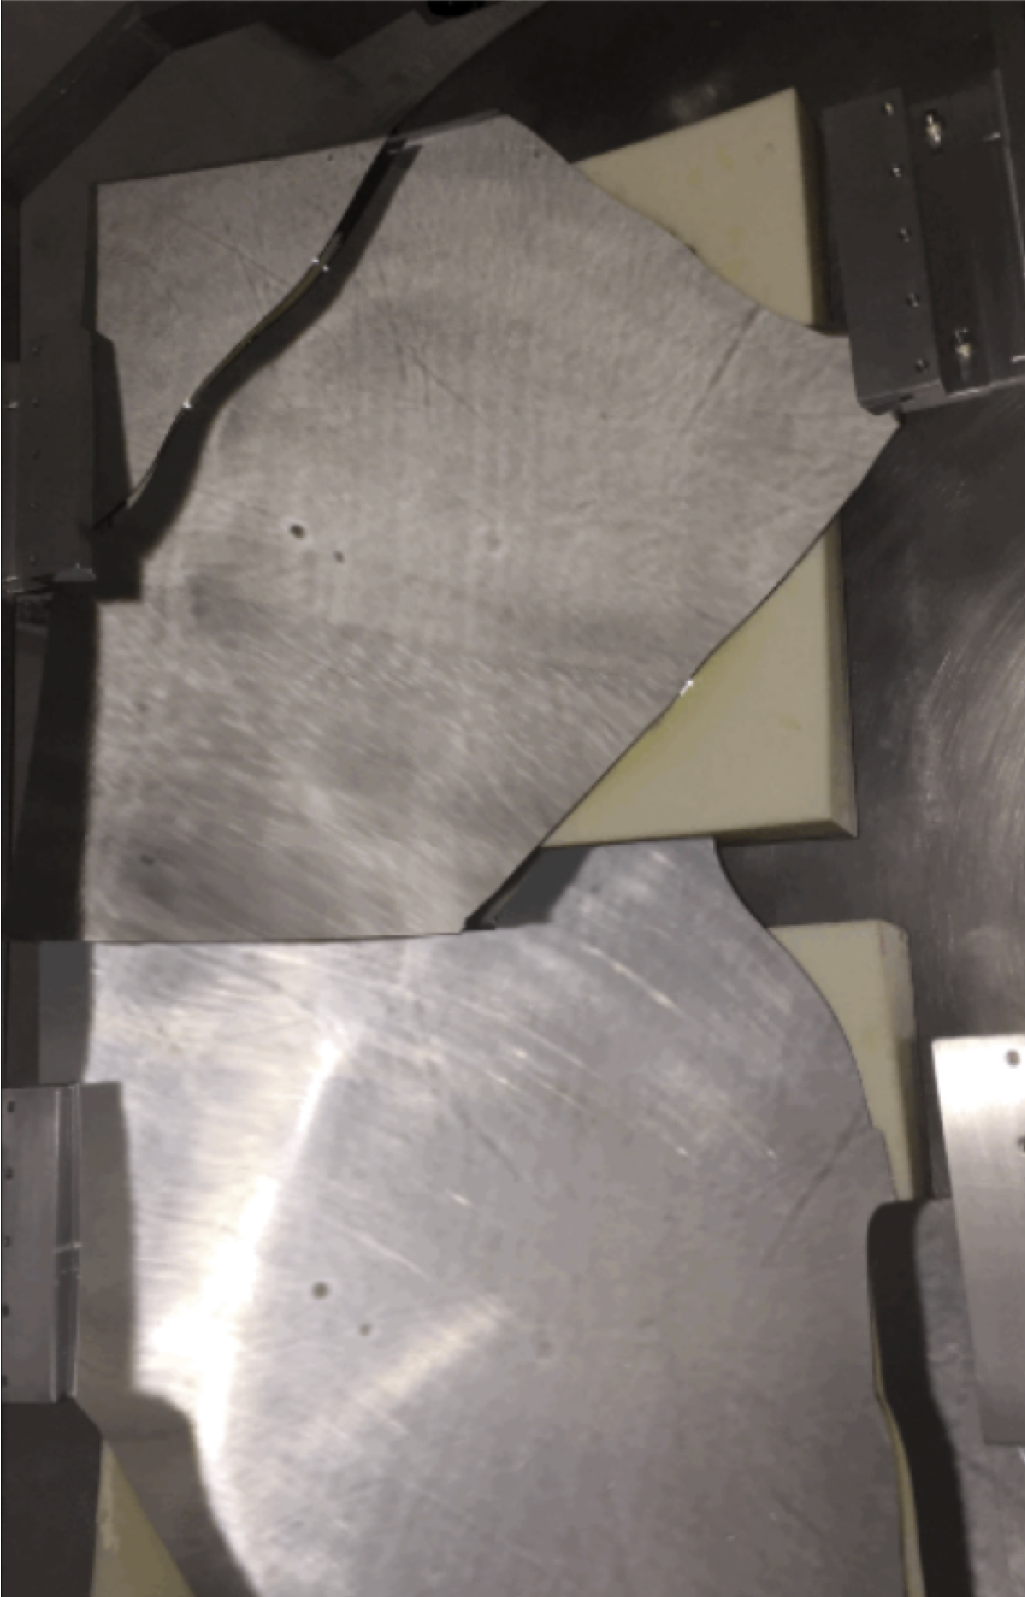
\includegraphics[width=0.6\textwidth]{chap4/hms_mirrors.png}
    \caption{
            A picture of the broken HMS Cherenkov mirrors taken after the
            detector was removed from the hut for repair.
            The mirrors' Rohacell supports are visible where portions of the
            mirrors have broken off.
            }
    \label{fig:hms_mirrors}
\end{figure}


Data shown in these figures are from defocused HMS run 1327.
Because the magnets were defocused, reconstruction of the
particles' momenta was not possible, so one cannot use the
track-normalized energy deposition to select electrons that should fire the
Cherenkov.
For this reason, the energy deposition divided by the spectrometer's central
momentum (a less precise version of track-normalized energy deposition)
was used.
A defocused run has the advantage of illuminating the spectrometer's entire
acceptance, allowing a full characterization of which regions of the acceptance
are negatively affected by the broken mirrors.

\begin{figure}[h]
    \centering
    \begin{subfigure}[b]{0.45\textwidth}
        \centering
        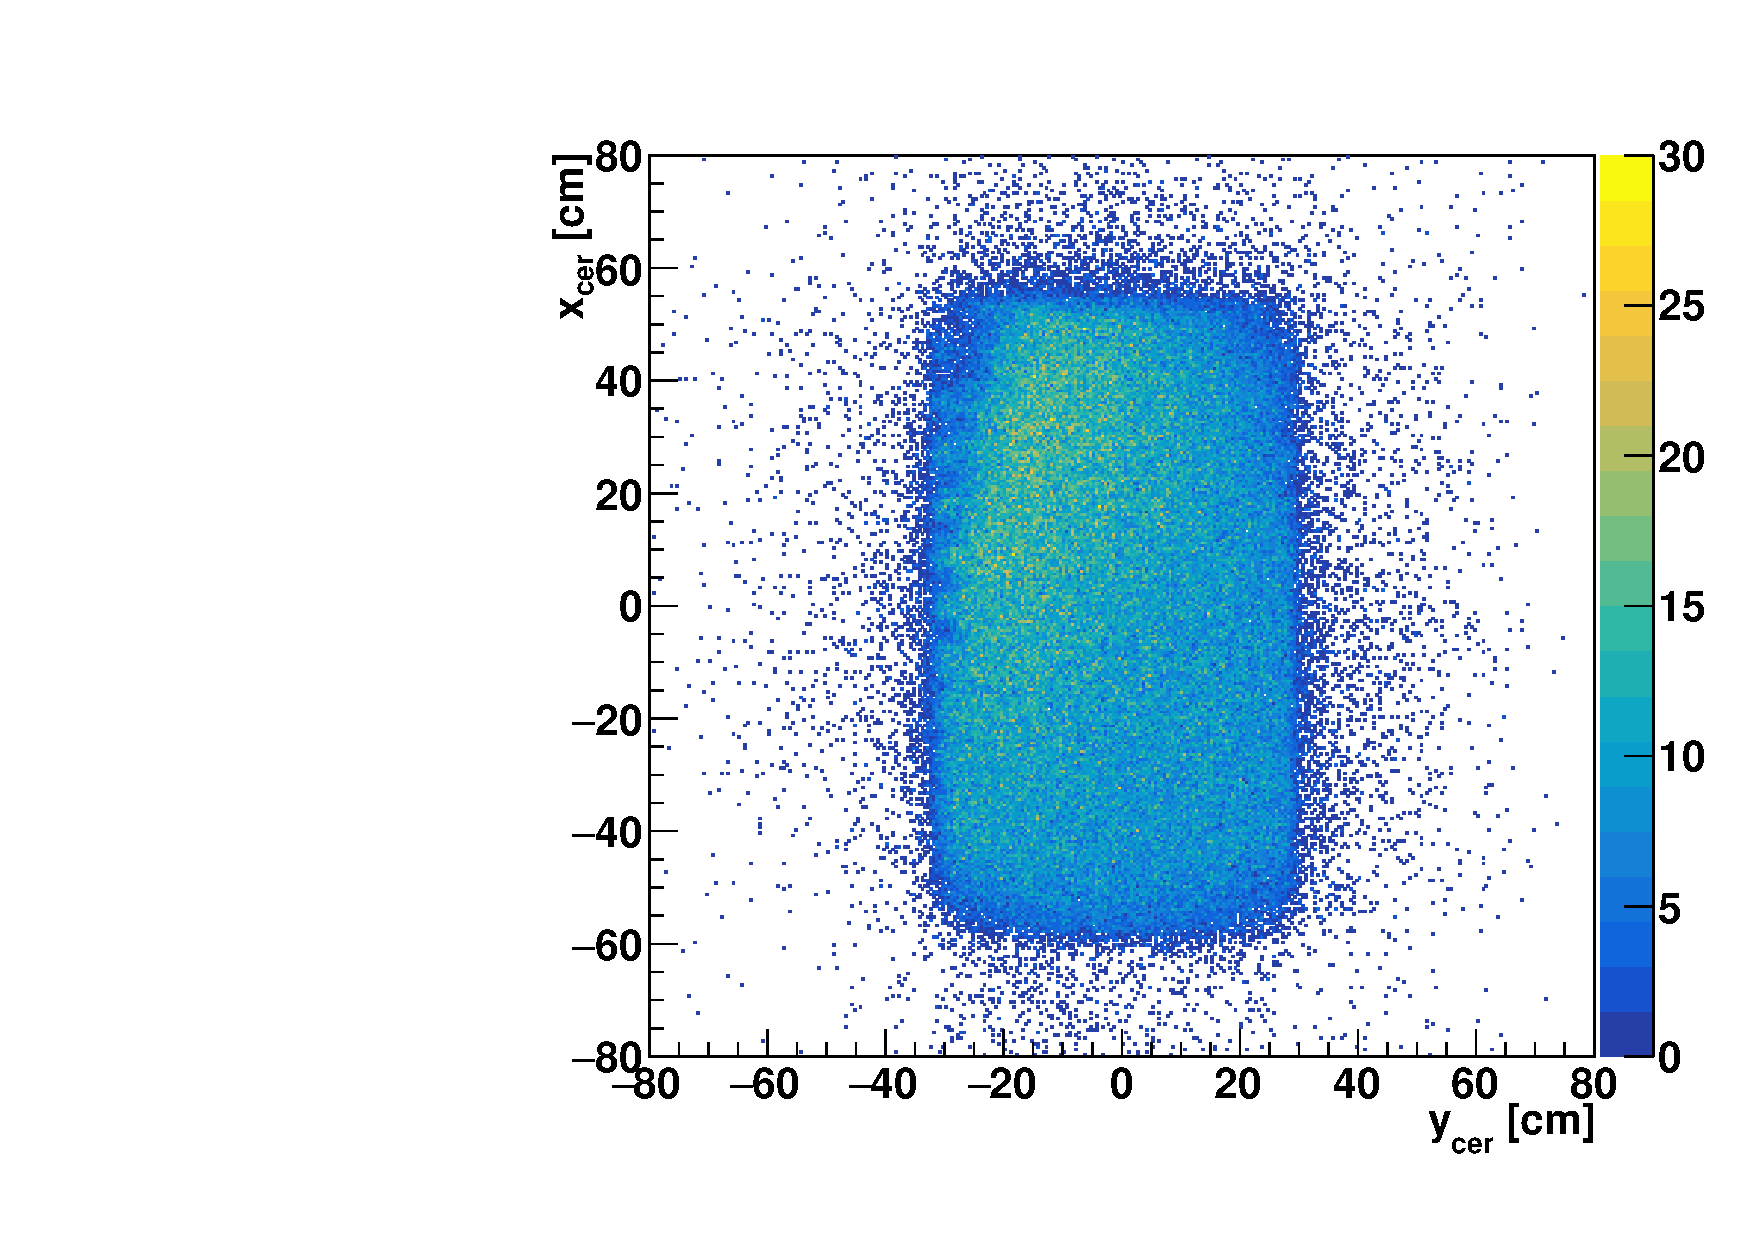
\includegraphics[width=\textwidth]{chap4/plot_scripts/hCer_should.pdf}
        % \caption{X plane}
        \label{fig:hms_mirror_should}
    \end{subfigure}
    % \hfill
    \begin{subfigure}[b]{0.45\textwidth}
        \centering
        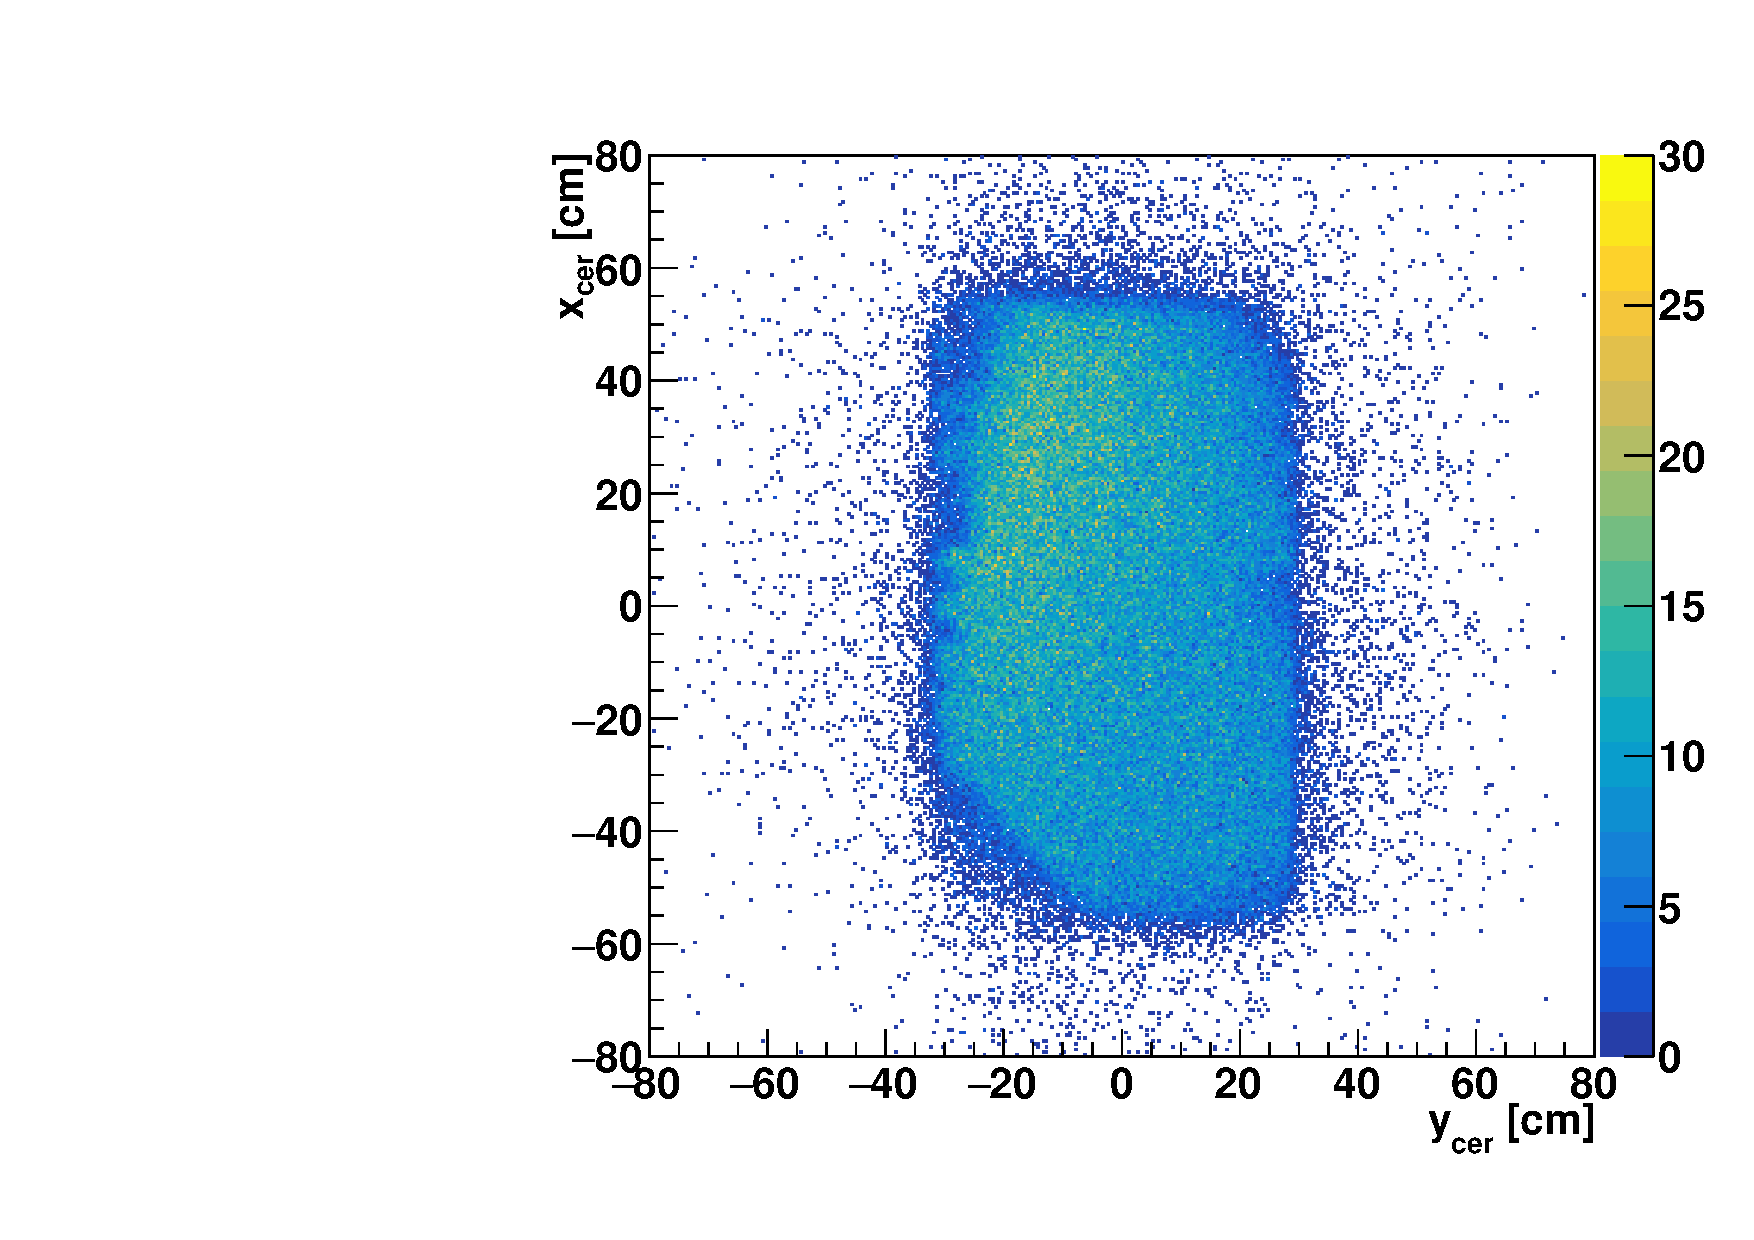
\includegraphics[width=\textwidth]{chap4/plot_scripts/hCer_did.pdf}
        % \caption{U plane}
        \label{fig:hms_mirror_did}
    \end{subfigure}
    \caption[
            The distribution of tracks projected to the HMS Cherenkov mirrors
            for events that should (left) and did (right) fire the Cherenkov.]{
            The distribution of tracks projected to the HMS Cherenkov mirrors
            for events that should (left) and did (right) fire the Cherenkov.
            Data shown are from defocused HMS run 1327.
            Events that should fire were selected by requiring the energy
            deposition in the HMS calorimeter normalized to the HMS central
            momentum to be between 0.9 and 1.1.
            No cuts were placed on $\beta$ or $\delta$.
            }
    \label{fig:hms_mirror_defocused_tracks}
\end{figure}

\begin{figure}[!h]
    \centering
    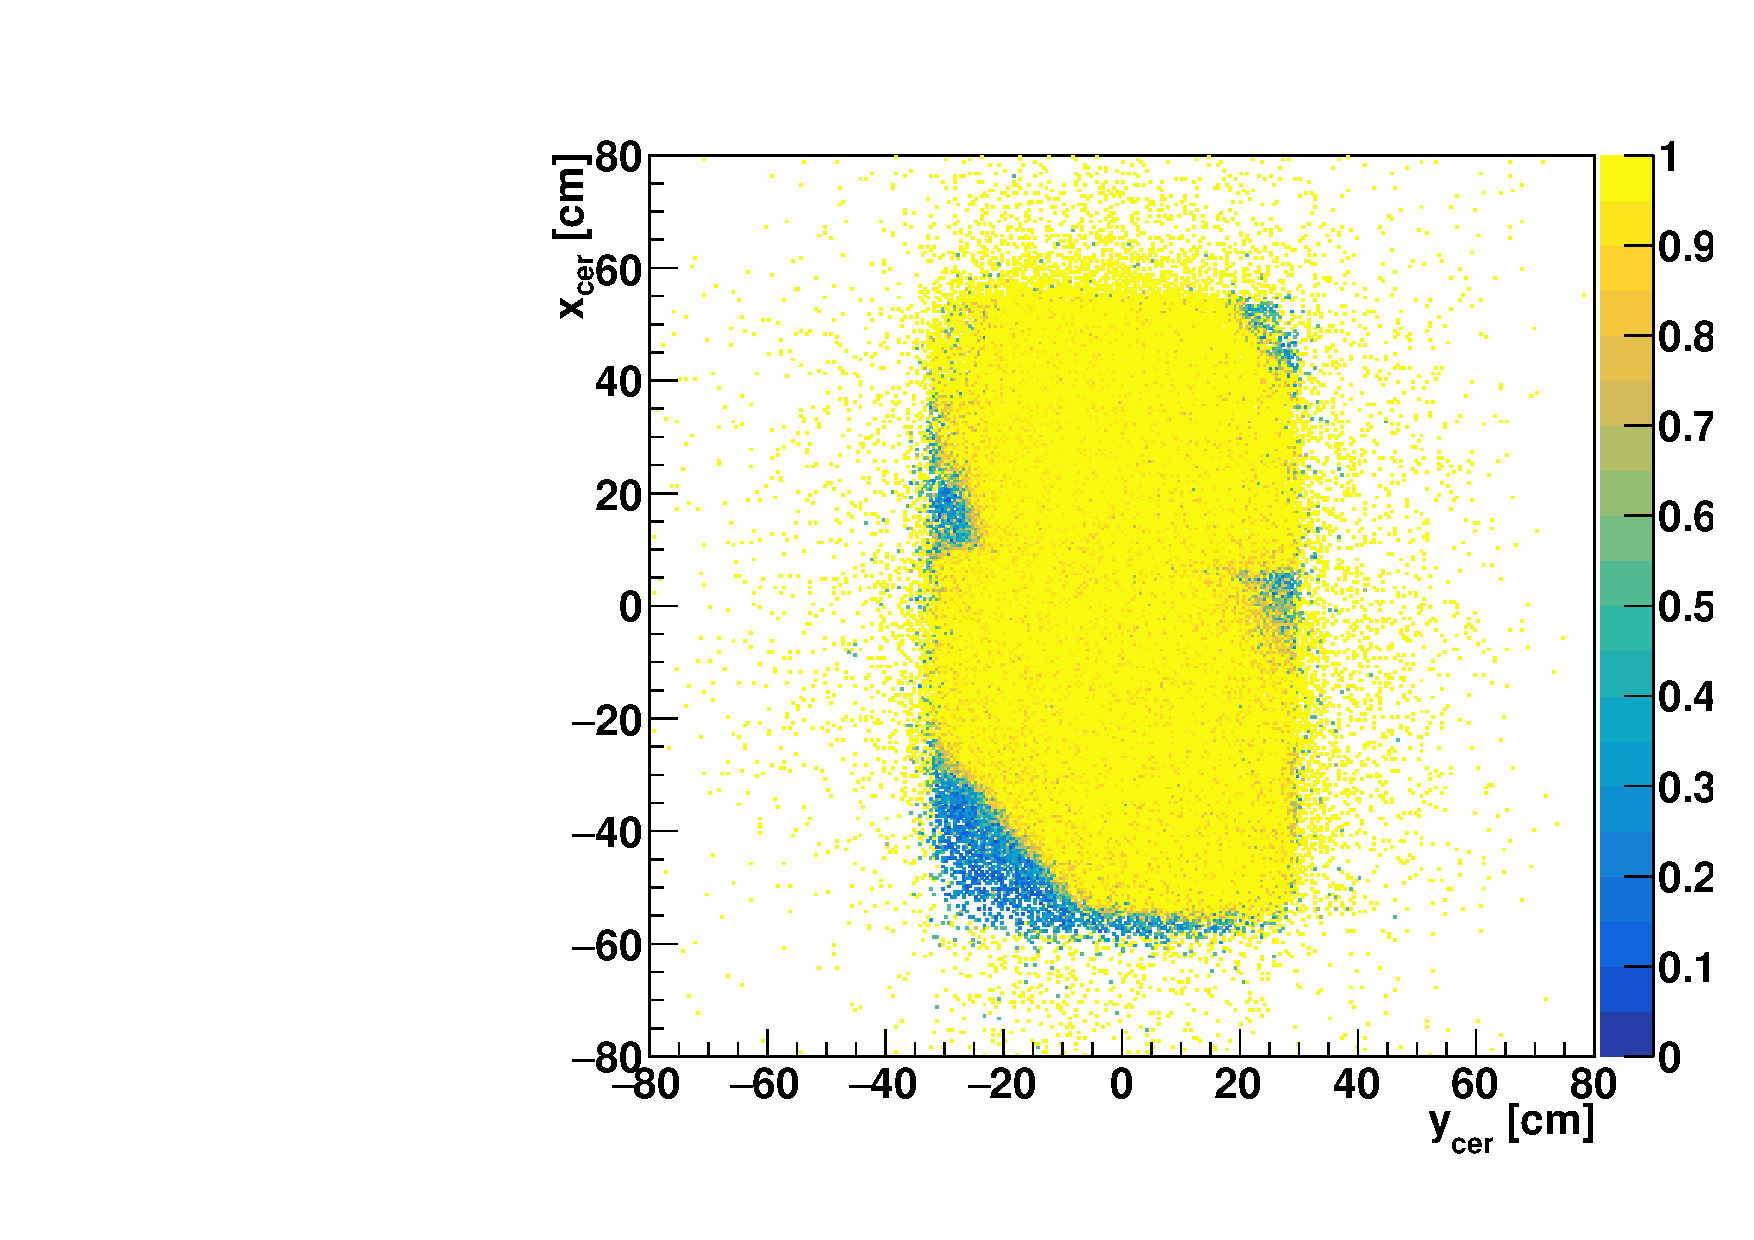
\includegraphics[width=0.6\textwidth]{chap4/plot_scripts/hCer_eff.pdf}
    \caption[
            The efficiency of the HMS Cherenkov, binned by track position
            projected to the Cherenkov mirrors.]{
            The efficiency of the HMS Cherenkov, binned by track position
            projected to the Cherenkov mirrors.
            The regions most affected by the broken mirrors are at large
            negative $x$ and $y$, large positive $x$ and $y$, and on the edges
            near the center of the dispersive direction $x$.
            }
    \label{fig:hms_mirror_efficiency}
\end{figure}

Fig~\ref{fig:hms_mirror_lh2_tracks} and Fig~\ref{fig:hms_mirror_c12_tracks}
show the distribution of track positions at the HMS Cherenkov mirrors for all
events that should fire the Cherenkov in our production
$Q^2=\SI{8.0}{\giga\electronvolt\squared}$ data.
This sample is selected using the same $C^{should}$ cut defined in
Table~\ref{tab:hcer_cuts} used to estimate the detector's efficiency.
Because the vast majority of our events lie in the central region of the
acceptance that is unaffected by the broken mirrors, it is sufficient to
include this effect as part of the overall efficiency estimate for this
detector.

\begin{figure}[!h]
    \centering
    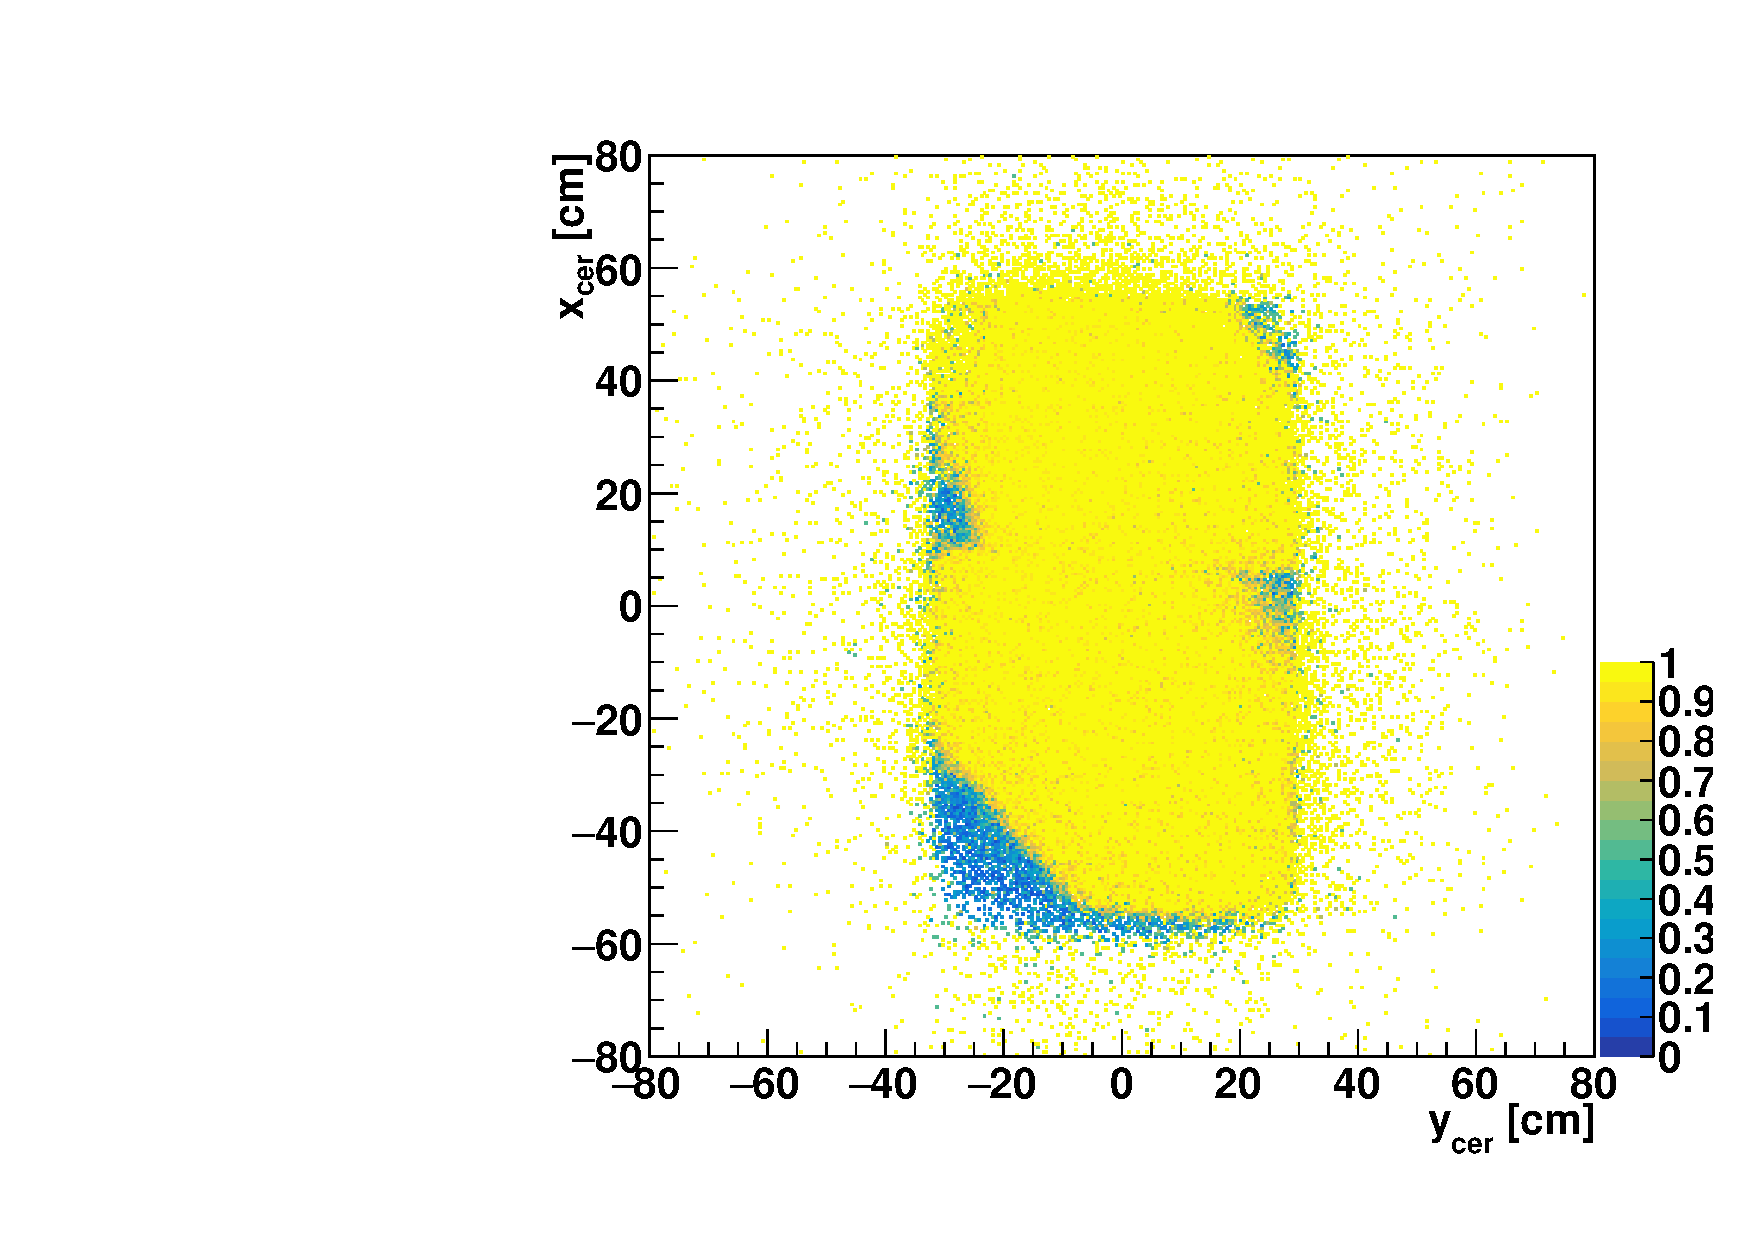
\includegraphics[width=0.6\textwidth]{chap4/plot_scripts/hCer_eff_short_pal.pdf}
    \llap{\raisebox{0cm}{
      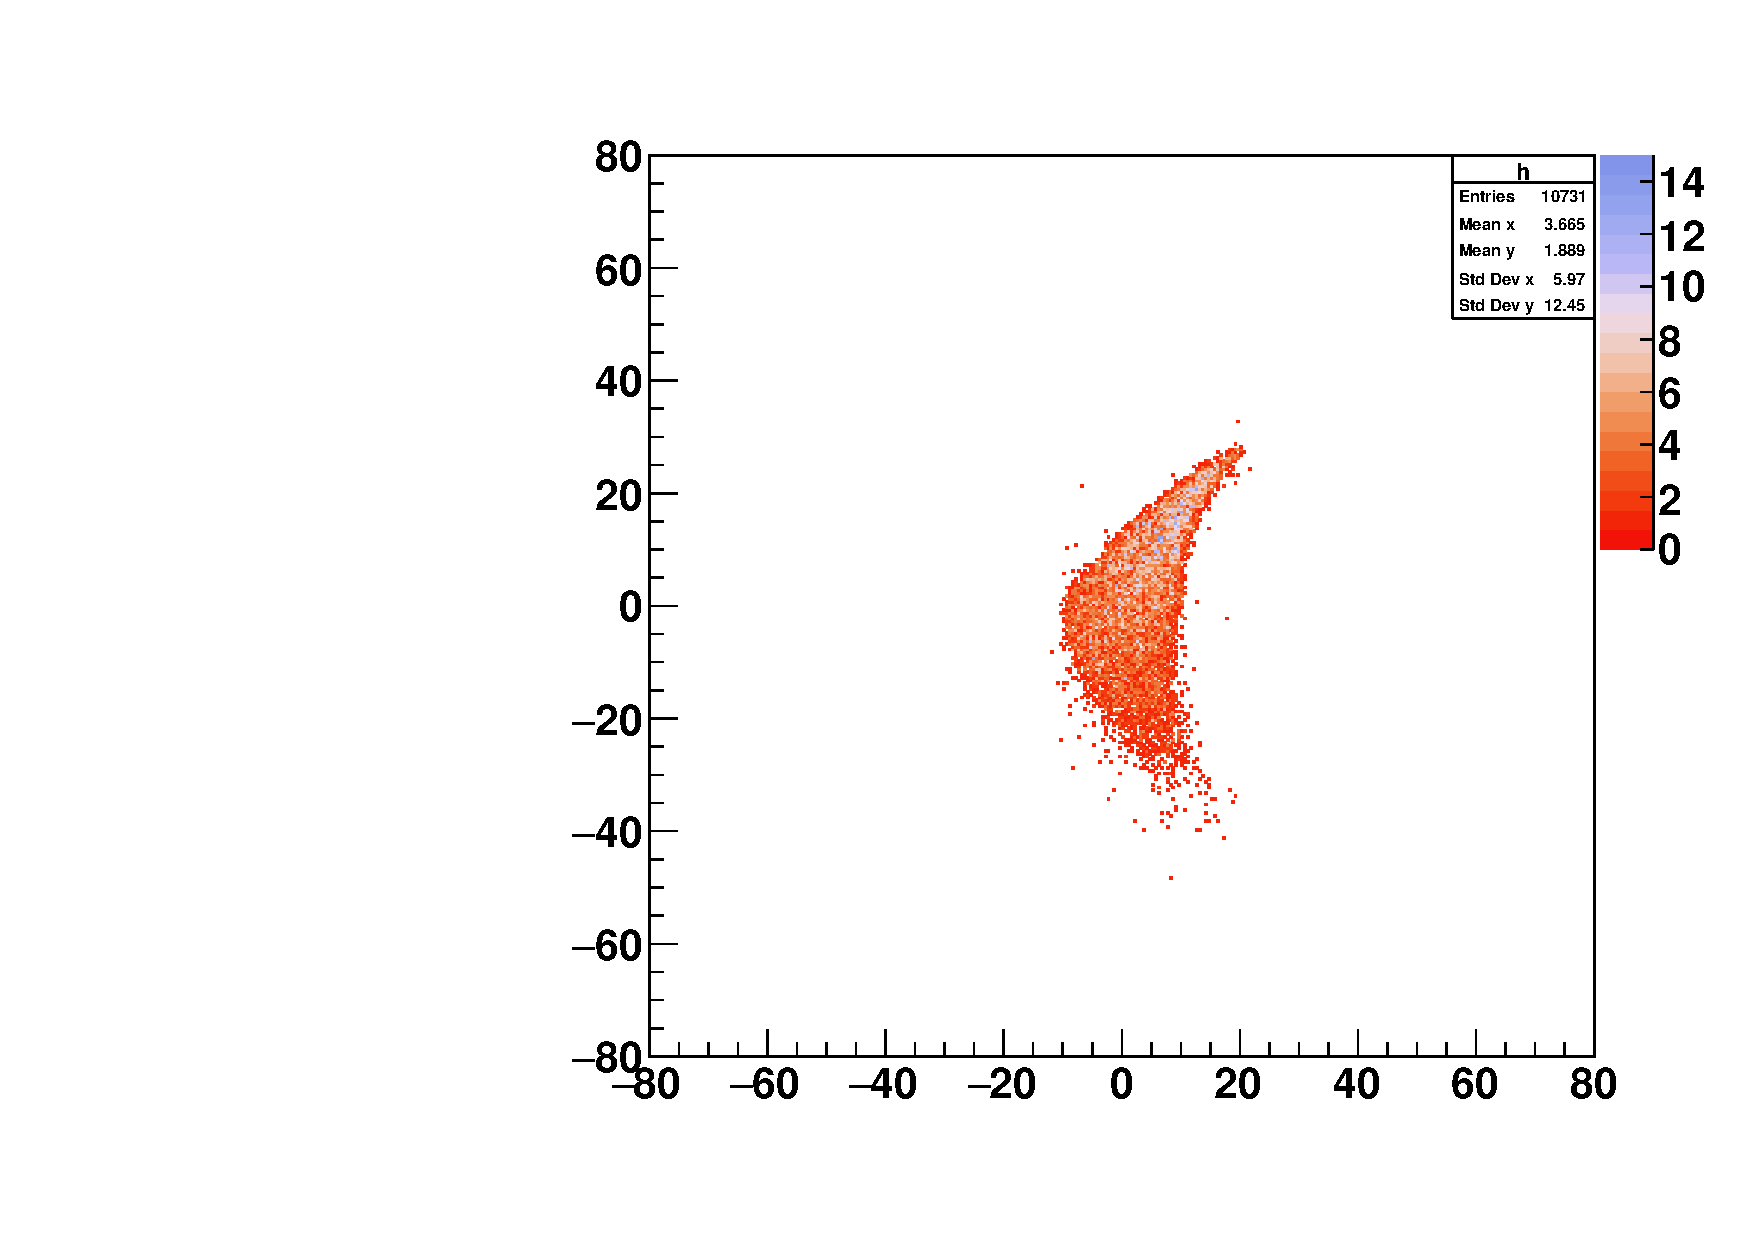
\includegraphics[width=0.6\textwidth]{chap4/plot_scripts/cherenkov_plots_coin_replay_production_LH2_8_0_smallcoll.pdf}
    }}
    \caption{
            The distribution of tracks projected to the HMS Cherenkov mirrors
            for our $Q^2=\SI{8.0}{\giga\electronvolt\squared}$ $H(e,e'p)$
            data is shown in red and lavender
            on top of the
            efficiency as a function of position in blue and yellow.
            }
    \label{fig:hms_mirror_lh2_tracks}
\end{figure}


\begin{figure}[!h]
    \centering
    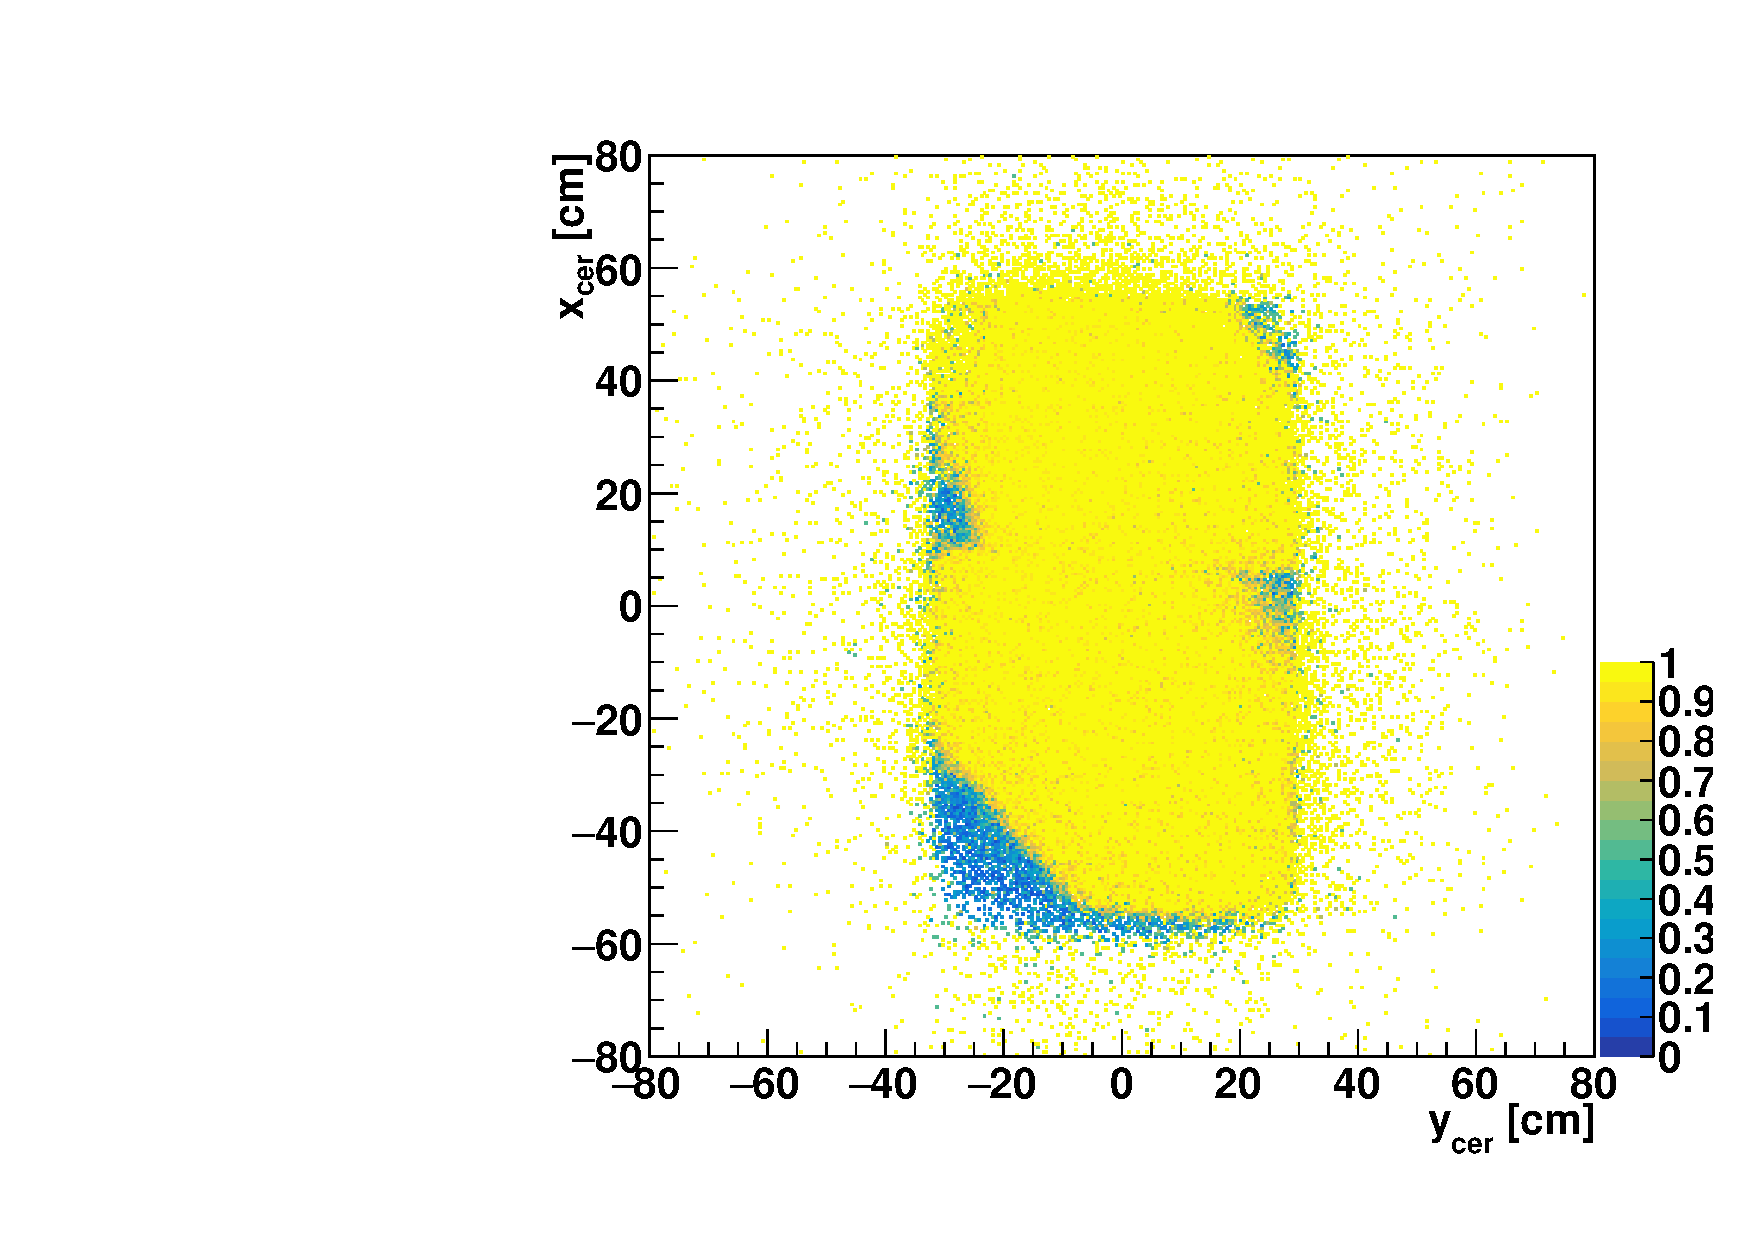
\includegraphics[width=0.6\textwidth]{chap4/plot_scripts/hCer_eff_short_pal.pdf}
    \llap{\raisebox{0cm}{
      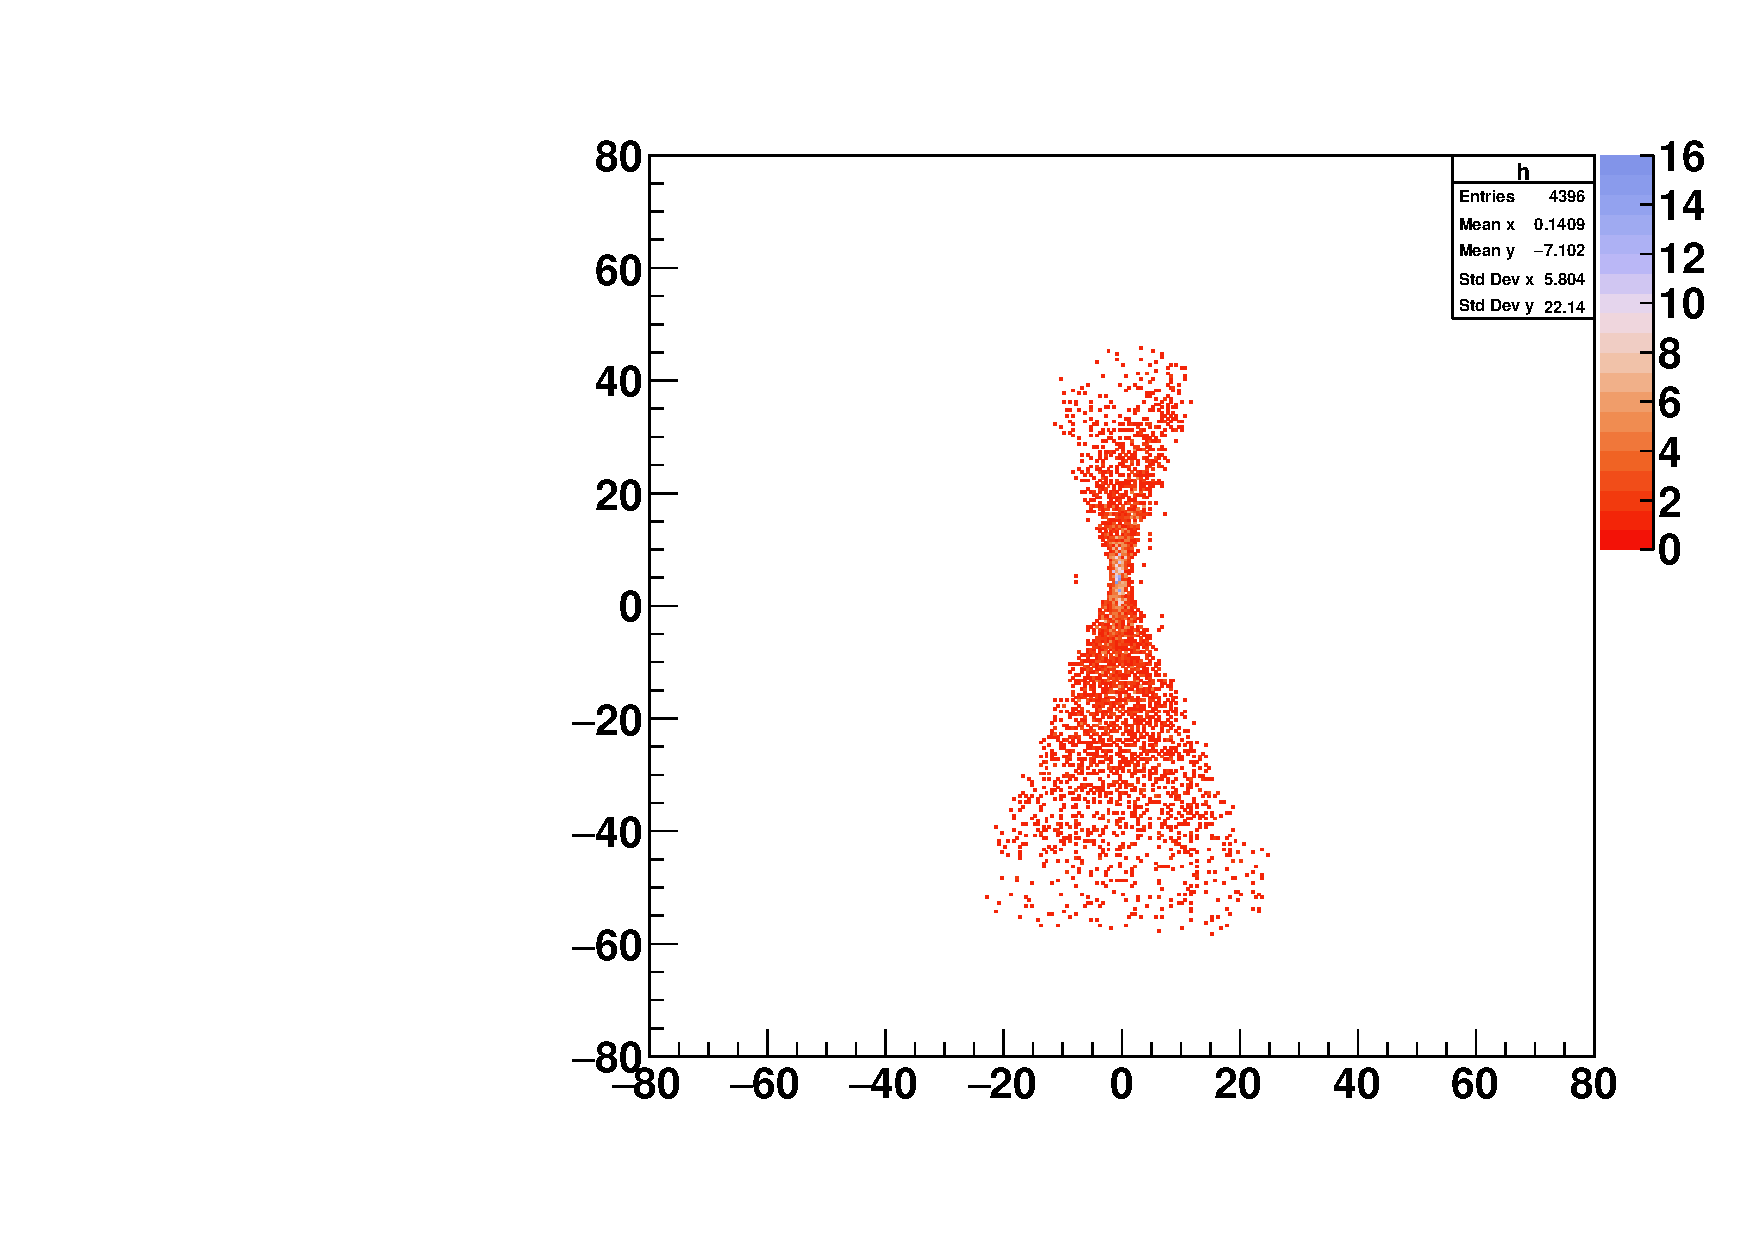
\includegraphics[width=0.6\textwidth]{chap4/plot_scripts/cherenkov_plots_coin_replay_production_C12_thick_8_0_smallcoll.pdf}
    }}
    \caption{
            The distribution of tracks projected to the HMS Cherenkov mirrors
            for our $Q^2=\SI{8.0}{\giga\electronvolt\squared}$ ${}^{12}C(e,e'p)$
            data is shown in red and lavender
            on top of the
            efficiency as a function of position in blue and yellow.
            }
    \label{fig:hms_mirror_c12_tracks}
\end{figure}


\subsection{SHMS Noble Gas Cherenkov}
The SHMS Noble Gas Cherenkov was used as a pion veto.
The SHMS central momenta used in this experiment range from
5.122 to \SI{8.505}{\giga\electronvolt}.
The pion threshold in this detector is \SI{4.65}{\giga\electronvolt} while the
the proton threshold is \SI{30}{\giga\electronvolt}, well above the range of
the SHMS magnets.
A set of protons that should not fire the Cherenkov
are selected using the cuts in Table~\ref{tab:pcer_cuts}.
A weighted efficiency is calculated as discussed in Section~\ref{sec:hcal_eff}

\begin{table}[h]
    \centering
    \caption{List of cuts used to estimate SHMS Noble Gas Chereknov efficiency.}
    \label{tab:pcer_cuts}
    %\begin{tabular}[t]{| c | l | l |}
    \begin{tabular}[t]{ c  l  l }
\specialrule{.1em}{.05em}{.05em}
                   &  Variables              &  Cut \\
\specialrule{.1em}{.05em}{.05em}
        \multirow{3}{*}{\makecell[ml]{$C^{should}$}}
        &  $\delta_{SHMS}$        &  -10.0 < P.gtr.dp \&\& P.gtr.dp < 10.0  \\ \cline{2-3}
        &  $\beta_{SHMS}$         &  P.gtr.beta < 1.4 \\ \cline{2-3}
        &  Good hodoscope time    &  P.hod.goodstarttime==1                 \\
\specialrule{.1em}{.05em}{.05em}
        \multirow{1}{*}{\makecell[ml]{$C^{PCer}$}}
        &  SHMS Cherenkov NPE     &  P.ngcer.npeSum<0.1                     \\
\specialrule{.1em}{.05em}{.05em}
    \end{tabular}
\end{table}

\subsection{Tracking}
The tracking efficiency $\epsilon_{track}$ is the probablity of hcana
reconstructing track based on signals wtih drift chamber wires when a particle
passes through the spectrometer.
The set of cuts used to select such events are listed in
Tables~\ref{tab:htrack_cuts} and~\ref{tab:ptrack_cuts}.
Events that should almost certainly have a good track candidate have
a reasonable value of $\beta$ estimated from time of flight
and
hits in hodoscope paddles in the ``fiducial region'' near the center of the
acceptance.
They will also not have ``too many'' drift chamber hits; particles in such
events may have grazed the edge of dipole window, creating an electromagnetic
shower, preventing hcana from reconstructing the track accurately.

The number of events with multiple candidate tracks in the HMS was small, so
the efficiency can be estimated by taken $N^{did}$ to be the number of events
that pass the cut $C^{should} \land C^{HTrack}$.
To correct for the larger amount of multitrack events in the SHMS, the
\textit{did} condition was adjusted to ensure that the golden track is located
in a central region of the acceptance and resulted in a reasonable focal plane
time.
Multitrack events were also not counted if they have ``too many'' hits on
negative side ADCs.
With this modification, the numerator in the SHMS tracking efficiency is the
number of events that pass the cut
$C^{should} \land (C^{PMultipleTrack} \lor C^{PSingleTrack}$),
where $\lor$ represents the logical operation \textit{or}.

\begin{table}[h]
    \centering
    \caption{List of cuts used to estimate HMS tracking efficiency.}
    \label{tab:htrack_cuts}
%    \begin{tabular}[t]{| c | l | l |}
      \begin{tabular}[t]{ c  l  l }
\specialrule{.1em}{.05em}{.05em}
&  Variables              &  Cut \\
\specialrule{.1em}{.05em}{.05em}
        \multirow{11}{*}{\makecell[ml]{$C^{should}$}}
        & Fiducial cut              & H.hod.goodscinhit==1 \\ \cline{2-3}
        & $\beta_{notrack}$         & \makecell{0.5 < H.hod.betanotrack \&\& \\
                                                H.hod.betanotrack < 1.4} \\ \cline{2-3}
        & Few hits in DC 1          & \makecell{(H.dc.1x1.nhit + H.dc.1u2.nhit + \\
                                                 H.dc.1u1.nhit + H.dc.1v1.nhit + \\
                                                 H.dc.1x2.nhit + H.dc.1v2.nhit) < 35} \\ \cline{2-3}
        & Few hits in DC 2          & \makecell{(H.dc.2x1.nhit + H.dc.2u2.nhit + \\
                                                 H.dc.2u1.nhit + H.dc.2v1.nhit + \\
                                                 H.dc.2x2.nhit + H.dc.2v2.nhit) < 35} \\ \cline{2-3}
        & SHMS Cherenkov NPE        & P.ngcer.npeSum<0.1 \\ \cline{2-3}
        & HMS Cherenkov NPE         & H.cer.npeSum>0 \\
\specialrule{.1em}{.05em}{.05em}
        \multirow{1}{*}{\makecell[ml]{$C^{HTrack}$}}
        & At least one track found  & H.dc.ntrack>0 \\
\specialrule{.1em}{.05em}{.05em}
    \end{tabular}
\end{table}

\begin{table}[h]
    \centering
    \caption{List of cuts used to estimate SHMS tracking efficiency.}
    \label{tab:ptrack_cuts}
%    \begin{tabular}[t]{| c | l | l |}
  \begin{tabular}[t]{ c  l  l }
\specialrule{.1em}{.05em}{.05em}
                   &  Variables              &  Cut \\
\specialrule{.1em}{.05em}{.05em}
        \multirow{11}{*}{\makecell[ml]{$C^{should}$}}
        & Fiducial cut              & P.hod.goodscinhit==1 \\ \cline{2-3}
        & Good hodoscope time       & P.hod.goodstarttime==1 \\ \cline{2-3}
        & $\beta_{notrack}$         & P.hod.betanotrack < 1.2 \\ \cline{2-3}
        & Few hits in DC 1          & \makecell{(P.dc.1x1.nhit + P.dc.1u2.nhit + \\
                                                 P.dc.1u1.nhit + P.dc.1v1.nhit + \\
                                                 P.dc.1x2.nhit + P.dc.1v2.nhit) < 25} \\ \cline{2-3}
        & Few hits in DC 2          & \makecell{(P.dc.2x1.nhit + P.dc.2u2.nhit + \\
                                                 P.dc.2u1.nhit + P.dc.2v1.nhit + \\
                                                 P.dc.2x2.nhit + P.dc.2v2.nhit) < 25} \\ \cline{2-3}
        & SHMS Cherenkov NPE        & P.ngcer.npeSum<0.1 \\ \cline{2-3}
        & HMS Cherenkov NPE         & H.cer.npeSum>0 \\
\specialrule{.1em}{.05em}{.05em}
        \multirow{1}{*}{\makecell[ml]{$C^{PSingleTrack}$}}
        & One track found           & P.dc.ntrack==1 \\
\specialrule{.1em}{.05em}{.05em}
        \multirow{17}{*}{\makecell[ml]{$C^{PMultipleTrack}$}}
        & \makecell{More than one track \\ found} & P.dc.ntrack > 1 \\ \cline{2-3}
        & \makecell{Few hits on negative \\ side ADCs} &
                \makecell{P.hod.1x.totNumGoodNegAdcHits<5 \&\& \\
                          P.hod.1y.totNumGoodNegAdcHits<5 \&\& \\
                          P.hod.2x.totNumGoodNegAdcHits<5 \&\& \\
                          P.hod.2y.totNumGoodNegAdcHits<5} \\ \cline{2-3}
        & Good focal plane time     &
                \makecell{-10 < P.hod.1x.fptime      \&\& \\
                                P.hod.1x.fptime < 50 \&\& \\
                          -10 < P.hod.1y.fptime      \&\& \\
                                P.hod.1y.fptime < 50 \&\& \\
                          -10 < P.hod.2x.fptime      \&\& \\
                                P.hod.2x.fptime < 50 \&\& \\
                          -10 < P.hod.2y.fptime      \&\& \\
                                P.hod.2y.fptime < 50} \\ \cline{2-3}
        & $\delta$                   & -15 < P.gtr.dp \&\& P.gtr.dp < 15 \\ \cline{2-3}
        & $y_{tar}$                  & -5 < P.gtr.y \&\& P.gtr.y < 5 \\ \cline{2-3}
        & $x'_{tar}$                & -0.2 < P.gtr.th \&\& P.gtr.th < 0.2 \\ \cline{2-3}
        & $y'_{tar}$                & -0.2 < P.gtr.ph \&\& P.gtr.ph < 0.2 \\
\specialrule{.1em}{.05em}{.05em}
    \end{tabular}
\end{table}

\subsection{Luminosity Scan}
At high beam currents and energies, energy deposition in liquid cryotargets
cause localized boiling.
This causes local drops in density which decrease measured charge-normalized
yields from what would be expected for a liquid target with constant density.
A beam current-dependent \textit{target boiling correction} can be extracted
with a luminosity scan, which consists of measuring charge-normalized yields
over a range of beam currents with the same spectrometer settings.
A linear fit of the drop in yield with increased current provides a
correction that can be used with production data at any beam current.

Table~\ref{tab:target_boiling_runs} lists the HMS and SHMS singles runs used to
study target boiling.
These runs were taken immediately before and after this experiment.
Both the HMS and SHMS were set at scattering angles of \SI{25}{\degree} and
central momenta of \SI{4.4}{\giga\electronvolt} to collect electrons scattered
from hydrogren and carbon targets.

\begin{table}[h]
    \centering
    \caption{List of runs used to study target boiling and the corresponding nominal beam currents.}
    \label{tab:target_boiling_runs}
%    \begin{tabular}[t]{| c | l | l | l |}
    \begin{tabular}[t]{ c  l  l  l }
\specialrule{.1em}{.05em}{.05em}
         Target          &  Current [\si{\micro\ampere}]  &  SHMS run  & HMS run\\
\specialrule{.1em}{.05em}{.05em}
        \multirow{7}{*}{\makecell[ml]{$LH_2$}}
        & 10 & 3210       & 2078,2080 \\ \cline{2-4}
        & 20 & 3211       & 2081 \\ \cline{2-4}
        & 35 & 3212, 3213 & 2082, 2083 \\ \cline{2-4}
        & 45 & 3214       & 2084 \\ \cline{2-4}
        & 55 & 3215       & 2085 \\ \cline{2-4}
        & 70 & 3207       & 2076 \\ \cline{2-4}
        & 80 & 3206       & 2075 \\
\specialrule{.1em}{.05em}{.05em}
        \multirow{1}{*}{\makecell[ml]{Aluminum Dummy}}
        & 40 & 3226 & 2096 \\
\specialrule{.1em}{.05em}{.05em}
        \multirow{3}{*}{\makecell[ml]{1.5\% ${}^{12}C$}}
        & 60 & 3223 & 2093 \\ \cline{2-4}
        & 50 & 3224 & 2094 \\ \cline{2-4}
        & 35 & 3225 & 2095 \\
\specialrule{.1em}{.05em}{.05em}
    \end{tabular}
\end{table}

The average of the normalized slopes and intercepts of the fits to SHMS and HMS
hydrogen runs was used as a correction to the production hydrogen yields of the
form
% TODO: confirm this number. It's what we have in the spreadsheet.
\begin{equation}
    f_{boil}(I_{mean})=1-0.000385I_{mean}
\end{equation}
where $I_{mean}$ is the mean beam current during the run whose yield is to be
corrected.

The slopes of fits to carbon yields were consistent with zero, as should be the
case for a solid target;
if the yields are appropriately corrected for rate-dependent effects (i.e.
deadtime and detector efficiencies) the yield should be independent of current.
The variation in carbon yields from the luminosity scan was used as an estimate
of the systematic uncertainty due to deadtime and detector efficiencies.

\subsection{Trigger}
Let $P_i$ be the efficiency of the $i$th hodoscope plane in one spectrometer.
This efficiency is estimated by taking tracks that point to the center of
the plane's paddles and counting how many times the paddle actually fires.
Because the triggers used in this experiment were formed by the coincidence of
three of 4 hodoscope planes, the trigger efficiency is given by the product of
the spectrometers' individual 3/4 efficiencies,
\begin{align}
    \epsilon_{hodo} = P_{3/4} =& P_{1} P_{2} P_{3} P_{4}+P_{1} P_{2} P_{3}\left(1-P_{4}\right)+P_{1} P_{2}\left(1-P_{3}\right) P_{4} \\
              &+P_{1}\left(1-P_{2}\right) P_{3} P_{4}+\left(1-P_{1}\right) P_{2} P_{3} P_{4}
\end{align}
This calculation is carried out by the THcHodoscope::TrackEff() method in
hcana and saved in the text report output saved when a run is
replayed.

\subsection{Livetime} \label{sec:livetime}
When a trigger is accepted, the DAQ system is unable to accept additional
triggers for a time determined by the gate widths of front end electronics and
the time it takes for CODA to write the event to disk.
The time during which the DAQ is unable to accept another event is referred to
as deadtime.
The inverse concept, livetime, refers to the total time that the DAQ is
\textit{not} occupied by processing incoming triggers.
The total livetime $TLT$ is a correction applied to the charge normalized yield
to account for events that are missed because of this phenomenon.

% TODO: edtm logic diagram
The EDTM (see Section~\ref{sec:edtm}) pulser allows an estimate of the total
livetime in a given run.
It sends regular pulses at a low frequency (\SI{3}{\hertz} in our experiment) at the
trigger logic level in the counting house.
By comparing the number of triggers that are accepted by the DAQ to the number
of pulses that are counted by the EDTM scaler, we can estimate the total
livetime as
\begin{equation}
    TLT = \frac{N_{EDTM,accepted}}{N_{EDTM,scaler}}
\end{equation}
where $N_{EDTM,accepted}$ is the number of events with a non-zero hit in the
EDTM TDC spectrum and $N_{EDTM,scaler}$ is the total number of EDTM triggers
counted by the EDTM scaler.
% TODO: Peter Bosted's correction. I don't understand his derivation.
% Let n be accepted, N be scaler count. Then L=n/N
% Let j be the current, and jc be the "cut current"
% Let f=j/jc
% Then Peter's correction is Lnew = (L-(1-f))/f
% The assumption here is that livetime is 100% when the beam is "off"
% i.e. below the cut value (typically a couple uA) used by hcana


% TODO: trigger rate figure
Because livetime should be dependent on trigger rate and the trigger rates
vary between our kinematic settings, we calculate a per-run livetime to
correct each run's yield.
Moreover, the EDTM system was not functional when we took our first set of data
for $Q^2$ of \SI{8}{\giga\electronvolt\squared}.
To estimate the livetime for these data, we performed a linear fit of the other
kinematics' $TLT$ dependence on SHMS 3/4 trigger rate and used this fit to
estimate the livetime for the $Q^2$=\SI{8}{\giga\electronvolt\squared} runs.

% TODO: LTE vs pTRIG1 (SHMS 3/4)

The computer livetime can be estimated as
\begin{equation}
    CLT = \frac{N_{phys,accepted}-N_{EDTM,accepted}}{N_{phys,scaler}-N_{EDTM,scaler}}
\end{equation}
The computer livetime for our data is negligible because CODA was configured to
only take coincidence events, whose rates were all quite low (below
\SI{6}{\hertz}) for all our kinematics.

% TODO: computer livetime vs pTRIG6

% TODO: add refs for Eric and Dave's slides

